%% This file is part of the spectroscopic_parallax project
%% Copyright 2018 the authors.

% To-do items
% -----------
% - make sure we address the sensibleness and generality of the linear model for the photometric space
% - Coryn's point that we should carefully explain how our model is geometric.
% - related: HWR's point that this is standardizeable candles, like the Ia SNe results.
% - related: Put in an explanation of WHY this works so well.
% - related: Put in an explanation of how it is that we aren't really modeling luminosity or distance but really just generating parallaxes.
% - does the model need a cute name, like The Swan?
% - check with WISE experts that we have the correct WISE photometry
% - we need an uncertainty estimate or noise model for our outputs.
% - general HWR point that we aren't putting in to the model any idea about how apparent magnitude varies with distance; this means that we rely on data for EVERYTHING.
% - write words about the setting of Lambda and the parallax offset (currently 0.0483 +/- 0.012 mas)
% - we have shown that outliers in sp - gaia tend to have large H-W2 or excess flux like in crowded regions, but there are some exceptions. Our error estimates are consistent with no intrinsic scatter if we use a robust chi-squared estimate. That is, chi-squared is dominated by outliers. We clipped the bad apogee spectral pixels at an error of 0.05 in normalized flux. Our uncertainty estimates are sensitive to this. The reader is asked to suck it.
% - write words about other linear models we have made or could make, probably in the discusssion.

\documentclass[modern]{aastex62}
\usepackage{amsmath}

%% Reintroduced the \received and \accepted commands from AASTeX v5.2
%\received{TBD}
%\revised{TBD}
%\accepted{TBD}
%% Command to document which AAS Journal the manuscript was submitted to.
%% Adds "Submitted to " the arguement.
%\submitjournal{AAS Journals}

\shorttitle{spectrophotometric parallax}
\shortauthors{hogg, eilers, rix}
%\watermark{kittens}

% text macros
\newcommand{\documentname}{\textsl{Article}}
\newcommand{\sectionname}{Section}
\newcommand{\equationname}{equation}
\newcommand{\code}[1]{\texttt{\detokenize{#1}}}
\newcommand{\foreign}[1]{\textsl{#1}}
\newcommand{\etal}{\foreign{et al.}}
\newcommand{\eg}{\foreign{e.g.}}
\newcommand{\acronym}[1]{{\small{#1}}}
\newcommand{\project}[1]{\textsl{#1}}
\newcommand{\apogee}{\project{\acronym{APOGEE}}}
\newcommand{\gaia}{\project{Gaia}}
\newcommand{\wise}{\project{\acronym{WISE}}}
\newcommand{\zmass}{\project{\acronym{2MASS}}}
\newcommand{\sdssiv}{\project{\acronym{SDSS-IV}}}
\newcommand{\sdssv}{\project{\acronym{SDSS-V}}}

% math macros
\newcommand{\T}{^{\mathsf{T}}}
\DeclareMathOperator*{\argmin}{argmin}
\newcommand{\logg}{\log g}
\newcommand{\BP}{{G_\mathrm{BP}}}
\newcommand{\RP}{{G_\mathrm{RP}}}
\newcommand{\gparallax}{\varpi^{(\mathrm{a})}}
\newcommand{\sparallax}{\varpi^{(\mathrm{sp})}}

% tweak the modern style -- trust in Hogg
\setlength{\parindent}{1.0\baselineskip}
\addtolength{\textheight}{0.5in}
\addtolength{\topmargin}{-0.3in}

\begin{document}\sloppy\sloppypar\raggedbottom\frenchspacing % trust in Hogg

\title{\textbf{%
Spectrophotometric parallaxes with \project{The Cygnet}:\\
Accurate distances for luminous red-giant stars
}}

\author[0000-0003-2866-9403]{David W. Hogg}
\affiliation{Center for Cosmology and Particle Physics, Department of Physics, New York University, 726 Broadway, New York, NY 10003, USA}
\affiliation{Center for Data Science, New York University, 60 Fifth Ave, New York, NY 10011}
\affiliation{Max-Planck-Institut f\"ur Astronomie, K\"onigstuhl 17, 69117 Heidelberg, Germany}
\affiliation{Flatiron Institute, 162 Fifth Ave, New York, NY 10010, USA}

\author[0000-0003-2895-6218]{Anna-Christina Eilers}
\affiliation{Max-Planck-Institut f\"ur Astronomie, K\"onigstuhl 17, 69117 Heidelberg, Germany}
\affiliation{International Max Planck Research School for Astronomy \& Cosmic Physics at the University of Heidelberg}

\author[0000-0003-4996-9069]{Hans-Walter Rix}
\affiliation{Max-Planck-Institut f\"ur Astronomie, K\"onigstuhl 17, 69117 Heidelberg, Germany}

\begin{abstract}\noindent
With contemporary infrared spectroscopic surveys like \apogee,
red-giant stars can be observed to distances and extinctions
at which geometric parallaxes are not precisely measured by \gaia.
Here we use the \apogee--\gaia\ overlap to train a purely linear model of
continuum-normalized \apogee\ spectroscopy
(plus \gaia, \zmass, and \wise\ photometry)
that predicts distance modulus (logarithmic parallax or distance)
for red stars with $0<\logg<2.2$.
The training makes use of a justified likelihood function for the \gaia\ parallaxes,
so that the training can be performed with full use of uncertainties and
without any cuts on parallax or parallax signal-to-noise ratio (not even any non-negative
requirements).
There are no physical inputs to the model; it is a pure regression designed
to accurately predict astrometric parallaxes.
The model includes an L1 regularization that zeros out the contributions of
most spectral pixels to the parallax estimates.
The training is performed
with leave-out subsamples such that no star's astrometry is used even indirectly in its
spectrophotometric parallax estimate.
The model is flexible enough---and has enough photometric information---to
correct for extinction by dust without any
input of explicit extinction or reddening estimates.
We re-label each star in the sample
with a new spectrophotometric parallax; this new parallax has an empirical (1-sigma)
uncertainty of 9~percent, which is more precise than the \gaia\ parallax
for the vast majority of targets.
Validation with globular and open clusters shows that the spectrophotometric parallaxes
are both accurate and precise.
These distance estimates open up great opportunities for
mapping the Milky Way disk with the next
generation of spectroscopic surveys, and especially \sdssv.
\end{abstract}

\keywords{%
methods:~statistical
 ---
techniques:~spectroscopic
 ---
catalogs
 ---
surveys
% ---
%parallaxes
 ---
stars:~distances
 ---
Galaxy:~disk
 ---
infrared:~stars
}

\section*{~}\clearpage
\section{Introduction} \label{sec:intro}

If we want to make precise kinematic and element-abundance maps
of the Milky Way disk out to large heliocentric radii,
and especially through the extinction to the other side of the Galactic Center, we will
need to make use of luminous red giants, and we will need to observe in
the infrared.
These arguments motivate the \apogee\ (CITE), \apogee-2 (CITE), and \sdssv\ (\citealt{sdssv})
projects, which take spectra in the infrared, and deliver detailed abundances
along the entire red-giant branch up to the tip.
The maps made with these data will reveal the dynamics of the Milky Way and its disk,
and show us how and where stars form, and how they migrate around (and out of) the
disk with time.

As we operate these spectroscopic surveys,
the \gaia\ Mission (CITE) has been revolutionizing our view of the disk.
It delivers good proper motions everywhere,
and extremely valuable parallax information
locally.
However, it does not deliver precise geometric parallaxes over a large fraction of
the disk, and certainly not in the dusty and crowded regions.
For these reasons, the value of \gaia\ in these infrared spectroscopy projects is not
to deliver distance information directly, but rather to calibrate stellar models,
which then deliver distance information through relationships between stellar
luminosities and spectral characteristics.

Luminous red-giant stars are valuable for mapping the Milky Way disk for a number
lf reasons, only one of which is their great luminosities (and hence brightnesses
even at large distance).
They are extremely common (frequent) stars, much more common than distance-indicating
stars like Cepheids.
They are produced by stellar populations at all metallicities and almost all ages,
so they can be found in all parts of the Galaxy.
They have temperatures and surface gravities such that it is
straightforward to spectroscopically measure metallicities,
detailed chamical abundances, and stellar parameters, including ages (\citealt{martig, nessage}).
The red-giant branch is photometrically near-orthogonal to reddening vectors by dust,
so they are easy to de-redden or dust-correct.
And finally, in physical models of red giants, their predicted luminosities are simple
functions of composition, surface gravity, temperature, and age.
Thus, if we can measure these properties of red giants, we can (in principle) predict
their luminosities and use them as standard candles.
That is---like type Ia supernovae---red giants are standardizable candles.

In this project, we develop purely data-driven techniques to predict
red-giant parallaxes or distances with spectroscopy and photometry.
Our method capitalizes on the point that red-giant stars are dust-correctable,
standardizable candles, but it makes no use whatsoever of any stellar interior,
stellar exterior, or dust-reddening models.
We only use these physical expectations about red giants to recommend
data features---inputs---for the data-driven model.
The data-driven method uses patterns in the observed data themselves
to discover the relationships between spectral features in the spectra of the stars,
photometry (including colors), and parallax (or distance).

Data-driven models are very often more accurate than physical models of stars
for this kind of work, because they have the flexibility to discover
regularities or offsets in the data that are not captured by the physical
models.
They do better than physical models when there are lots of training data
with properties that are good for performing regressions.

Simple data-driven models (like the ones we will employ here)
suffer from many limitations for this kind of work:
Because they are constrained only by the data, and not physical law,
they can learn relationships that we know
to be physically unlikely, and (by the same token) they can't benefit from our
physical knowledge.
They are required, in some sense, to spend some of the information in the data on
learning physical laws or relationships.
Not all of the information in the data is being used
optimally when we ignore our physical models.
Relatedly, they are not (usually) interpretable or generalizable:
A data-driven model trained with one kind of data can not usually be used in another
context with very different input data.
And the internal properties of the model are not useful, in general, for improving
our understanding or intuition about the astrophysics in play.

All that said, our goal here is to produce a precise mapping tool for surveys
like \apogee\ and \sdssv.
So we will take the limitations of the data-driven models in exchange for their
performance.
This work builds on the success we have seen in building other kinds of
data-driven tools for  stellar spectroscopy, for example to measure stellar
parameters (\citealt{cannon}), abundances (\citealt{ho, casey, nessdopp}),
and masses and ages (\citealt{nessage}).

There is a huge range of complexity or capacity in data-driven
models, from linear regressions (what we use here) to the most advanced machine-learning
methods (like deep neural networks).
In this work we stay on the low-complexity side of this.
We do not want to face the (literally combinatoric) choices in model structure that
advanced methods bring.
And we want to control or understand the smoothness or flexibility of the model.
Deep networks can model extremely complex function spaces, which is good in some
contexts, but bad when you know that the functional dependencies you hope to
model are smooth:
In that case, much of the information in the data can get spent on learning the
smoothness of the function.

What follows is a regression:
We use \gaia\ measurements of parallax to learn relationships between 
the spectroscopic and photometric properties of stars and their parallaxes.
We then use that learned model to estimate improved parallaxes for stars with
poor (or no) \gaia\ measurements.
This regression is very sensitive to certain aspects of the data or experimental
design..
One is that we will do far better with the regression if we have an accurate
model for noise process in the \gaia\ data.
For this reason, we make use of a justifiable likelihood function for the
\gaia\ astrometry (\citealt{gaialf}).
Another is that regressions can be strongly biased if we have a bad selection function
or data censoring.
This means that we cannot apply cuts to the \gaia\ astrometry or signal-to-noise
unless those cuts are correctly accounted for in our generative model for the
data sample.
Below, we will make no such cuts. That means that our training step has the odd
property that much of the training data is low in signal-to-noise and many of the
training parallax measurements are even negative!
The fact that we are using a justified likelihood function ensures that these
data will only affect the model in sensible and justifiable ways.
The alternative---cutting to high signal-to-noise data---is the more traditional
approach, but it leads to biased inferences (unless the cuts are included correctly
in the likelihood function).
The method in which we make no cuts and keep an umodified, justified likelihood function
is unbiased, and simple.

\section{Assumptions of the method}\label{sec:assumptions}

Our position is that a methodological technique is correct inasmuch as
it delivers correct or best results \emph{under its particular assumptions}.
In that spirit, we present here the assumptions of the method
explicitly.
We will return to these assumptions in the Discussion section below,
to address the costs and benefits of each in more depth.
\begin{description}
\item[features] Perhaps our most fundamental assumption is that the parallax
of a star can be predicted from the features we provide, which are
the full set of (pseudo-continuum-normalized) pixels from the \apogee\ spectrum,
plus the $G$ and $(\BP-\RP)$ photometry from \gaia,
plus the $J$, $H$, and $K_s$ photometry from \zmass\ (\citealt{zmass}),
plus the $W_1$ and $W_2$ photometry from \wise.
That is, we assume that these spectrophotometric \emph{features} are sufficient
to predict the parallax in the face of variations in stellar
age, evolutionary phase, composition, and other parameters, and also interstellar
extinction.

\item[good features] We assume that the spectrophotometric features are known for
each star with such high fidelity (both precision and accuracy) that we do not
need to account for errors or uncertainties or biases in the features.
That is, we assume that the features are substantially higher in signal-to-noise than the
quantities we are trying to predict; in particular we are assuming that the photometry
and the spectroscopy is better measured than the astrometry.
This is true for most features for most stars, but it does not hold universally.

\item[representativeness] We assume that the training set constructed from the overlap
of \gaia\ and \apogee\ data sets constitutes a representative sample of stars,
sufficiently representative to train the model for all other stars.
Although this assumption is not terrible, it has a weakness:
The stars at greatest distances and greatest local (angular) stellar crowding have
the least precise \gaia\ parallax measurements, and therefore will effectively get
less weight in the fits performed to train the model.

\item[sparsity] We expect that only a small subset of the full complement of
\apogee\ spectral pixels will be relevant to the prediction of parallax
(the spectrophotometric parallax).
That is, we expect that many of the pixels will or ought to get no weight in the
final model that we use to predict luminosities and distances.

\item[linearity] Perhaps the most restrictive assumption of this work is that
the logarithmic parallax (or, equivalently, the distance modulus) 
can be predicted as a \emph{completely linear function} of
the chosen features. We are only assuming this linearity in a small range of stellar
surface gravity $\logg$, but this assumption is strong, and limits strongly the
flexibility or capacity of the model.
We make it to ensure that our method is easy to optimize, and the results are easy
to interpret.

\item[likelihood] We assume that the \gaia\ parallaxes are generated by a particular
stochastic process, in which the difference between the \gaia-Catalog parallax (plus
a small \gaia-recommended offset; \citealt{lindegren}) and the true parallax is effectively drawn from a
Gaussian with a width set by the \gaia-Catalog uncertainty on the parallax.
This is the standard assumption in all properly probabilistic \gaia-Mission inferences
to date, but it subsumes a number of related assumptions, like that the \gaia\ noise
model is correct, that the stars are only covariant at negligible levels, and that
there are no significant outliers or large-scale systematics.
\end{description}

In addition to making the above assumptions, we also avoid various practices
with the data that are tempting but lead to strong biases.
For example, we never cut on \gaia\ parallax or parallax signal-to-noise.
The common practices of cutting to parallaxes that are good to 20~percent,
or Catalog parallaxes that are positive, or parallaxes that are smaller or
larger than something, are all practices that will bias results on stellar
collections.
That is, if you cut on parallax or parallax signal-to-noise and you subsequently
take an average of parallaxes for some population, or perform a regression (as we
do here), the results of that average or regression will be strongly biased.
We never cut on parallax or parallax signal-to-noise.
By using a justifiable likelihood function (the ``likelihood'' assumption above),
we can use all of the \gaia\ parallaxes without the low signal-to-noise and
negative parallaxes causing trouble for our regressions, and without the biases
that enter when cuts are made.

Along similar lines, we never assume that the distance is the inverse of the
measured parallax.
In what follows, a star's distance is a latent property of the star, which generates
the \gaia\ Catalog parallax through a noisy process (again, this is
the ``likelihood'' assumption above).
We never take the inverse or the logarithm of the measured parallax at any time.
This is related to the no-cuts point above:
If you take the inverse or logarithm of the parallax, you can't operate safely
on the negative and low signal-to-noise parallaxes, which in turn will require
making cuts on the sample, which will in turn bias the results.

Finally, we never use Lutz--Kelker corrections (\citealt{lk}) or distance
posteriors (\eg, \citealt{calj}). These both involve (implicit or explicit) priors on 
distance.
When multiple stars are combined as we combine them here (below),
use of distance posteriors instead of parallax likelihoods is not just
unjustified, but it also leads to an
effective raising of the distance prior to an enormous power.
That is, the effective prior on a $N$-star inference performed naively
with distance posteriors (made with a weak prior) can end up
bringing into the inference an \emph{exceedingly
strong prior}.
Therefore we don't use any prior-contaminated parallax or distance
inputs to the inference.

\section{Method}

There are not many choices
for building a model of the stars that is both justifiable probabilistically
and consistent with the assumptions stated in the previous \sectionname.
Here we lay out the model and methodology.
We apply the method to real data in the following {\sectionname s}.

The model and log-likelihood function can be expressed heuristically as
\begin{eqnarray}
\gparallax_n &=& \exp(\theta\cdot x_n) + \mbox{noise}
\\
\chi^2(\theta) &\equiv& \sum_{n=1}^N \frac{[\gparallax_n - \exp(\theta\cdot x_n)]^2}{\sigma_n^2}
\quad ,
\end{eqnarray}
where
$\gparallax_n$ is the \gaia\ measurement (adjusted; see below) of the astrometric parallax of star $n$,
the model is that the logarithm of the true parallax
can be expressed as a linear combination of the components
of some $D$-dimensional feature vector $x_n$,
$\theta$ is a $D$-vector of linear coefficients,
$\sigma_n$ is the \gaia\ estimate of the uncertainty on the parallax measurement,
and $\chi^2(\theta)$ is (twice) the negative-log-likelihood for the parameters $\theta$
under the assumption of known Gaussian noise and
that there are $N$ independently measured stars $n$.
The feature vector $x_n$ contains photometry in a few bands, and all 7400-ish pixels
in the pseudo-continuum-normalized \apogee\ spectrum, so $D$ is on the order of 7400.

In addition, we assume that many entries in the parameter $D$-vector $\theta$ will be zero
(the ``sparsity'' assumption).
In order to encourage this, we optimize not $\chi^2$ but a regularized objective function
\begin{eqnarray}
\hat{\theta} &\leftarrow& \argmin_{\theta}\left[\frac{1}{2}\,\chi^2(\theta) + \lambda\,||P\cdot\theta||_1^1\right]
\label{eq:objective}\quad ,
\end{eqnarray}
where
$\lambda$ is a regularization parameter,
$P$ is a projection operator that selects out from the $\theta$ vector only those components
that pertain to the \apogee\ spectral pixels,
and $||y||_1^1$ is the L1-norm or sum of absolute values of the components of $y$.
This kind of regularization adds a convex term to the optimization and leads to
sparse optima.
The $P$ operator makes it such that we only regularize the components of $\theta$ that multiply
the spectral pixels; we ask for the spectral model to be sparse but we don't ask for the photometric
model to be sparse.
We set the value of $\lambda$ by a 
very coarse cross-validation.

This optimization is not convex---there are multiple optima in general.
In particular, there is a large, degenerate, pathological optimum where
the exponential function underflows, all parallaxes are predicted to vanish,
and there is no gradient of anything with respect to the parameter $D$-vector $\theta$.
This large, bad optimum (it is a local, not global, optimum) must be avoided in optimization.
In practice we avoid it by optimizing first for the very highest signal-to-noise
(in astrometric parallax) Training Set stars, and then use that first optimum as a
good first guess or initialization for the full optimization.
This method works because in the limit of high signal-to-noise, the problem asymptotically approaches
the convex problem of L1-regularized linear least-square fitting.
Optimization is performed with \code{scipy.optimize} \acronym{L-BFGS-B}.

Once the model is optimized, the output of the model is a prediction of the parallax,
or really what we will call the \emph{spectrophotometric parallax}.
This spectrophotometric parallax
$\sparallax_m$ for any star $m$ in the validation or test set is
assigned according to
\begin{eqnarray}
\sparallax_m &\leftarrow& \exp(\hat{\theta}\cdot x_m)
\quad ,
\end{eqnarray}
where
$\hat{\theta}$ is the optimal parameter vector according
to \equationname~(\ref{eq:objective}),
and
$x_m$ is the feature $D$-vector for star $m$.
Thus the model can be trained on a training set of stars and applied to make
predictions for a validation set or a test set.
The only requirements are that every test-set object $m$  must have a full feature
vector $x_m$ just as every training-set object $n$ must have a full feature
vector $x_n$.

One final detail: We perform all of the fitting in a two-fold train-and-test framework,
in which the data are split into two disjoint subsets, A and B.
The model trained on the A data is used to predict or produce
the spectrophotometric parallaxes $\sparallax_m$ values (and hence
the distances and parallaxes) of the B data,
and the model trained on the B data is used to 
produce the $\sparallax_m$ values of the A data.
This ensures that, in the estimate of any individal star's
parallax, none of the \gaia\ data pertaining to that star were used.
This makes the parallax estimates from the spectrophotometric feature vectors
$x_m$ statistically independent of the \gaia\ parallax measurements.
They are not independent globally---\gaia\ data were used to train the model---but
each star's spectrophotometric parallax estimate is independent
of the astrometric estimate from \gaia\ on a star-by-star basis.

\section{Data}

We take the \apogee\ (\citealt{aapogee, wapogee, apogee}) spectral data
from \sdssiv\ (\citealt{sdssiv}) \acronym{DR14} (\citealt{dr14}).
Because we want to make a purely linear model, which has very little capacity,
we restrict our consideration to a small region in stellar parameter space.
We cut the \apogee\ data down to the range $0<\logg<2.2$, which isolates
stars that are more luminous than the red clump.
The \apogee\ pipeline (\citealt{aspcap})
values of surface gravity $\logg$ (which we use) have uncertainties but
this cut leads to a clean sample of luminous red giants, and it is a cut
that is only on spectral properties of the stars (and not photometry nor astrometry).

From the \apogee\ data on these low-gravity stars, we take the spectral pixels,
of which there are 7405 (after cutting out pixels that rarely or never get data),
on a common rest-frame wavelength grid.
That is, every \apogee\ star is extracted on (or interpolated to)
the same wavelength scale.
In detail, we obtain the
the \apogee\ spectral pixels from the pipeline-generated \code{aspcapStar} files.
We then pseudo-continuum-normalize the spectra according to the procedure developed
in \project{The~Cannon} (\citealt{cannon}):
That is, the pseudo-continuum is a spline fit to a set
of pixels chosen to be insensitive to stellar parameters.
We use as our spectral data the normalized spectral pixel values.

Because the \apogee\ target selection is based on \zmass\ (\citealt{zmass}),
every \apogee\ star also comes with \zmass\ photometry.
That is, for each star $n$,
we have \zmass\ near-infrared photometry $J_n$, $H_n$, and $K_n$.

We used the \gaia\ Archive (\citealt{gaiaarchive})
official matches (\citealt{xmatch}) to match the \apogee+\zmass\ stars
to the \wise\ Catalog (HOGG CITE),
according to the \gaia\ Archive internal match criteria.
This gives, fore each matching star $n$,
mid-infrared photometry $W_{1n}$ and $W_{2n}$ at 3.6 and 4.5\,$\mu$m
In detail we use the \code{w1mpro} and \code{w2mpro} Catalog entries.

We match this full-match catalog to the \gaia\ \acronym{DR2} (HOGG CITE)
using the \gaia\ Archive official match (given the \zmass\ IDs).
We take from the \gaia\ \acronym{DR2} Catalog the photometric data
$G_n$ (\code{phot_g_mean_mag}),
$\BP_n$ (\code{phot_bp_mean_mag}),
and $\RP_n$ (\code{phot_rp_mean_mag}),
which will become part of the feature vector $x_n$.

We need complete feature-vector information for all stars.  For this
reason, we define the Parent Sample to be the set of all stars that
meet the \apogee\ and \gaia\ cuts and also
have the complete set of photometry: $G_n$, $\BP_n$, $\RP_n$, $J_n$,
$H_n$, $K_n$, $W_{1n}$, and $W_{2n}$ and also an \apogee\ spectrum.
In addition, we applied two light color cuts to remove stars with obviously
contaminated or outlying photometry:
\begin{eqnarray}
(J_n - K_n) &<& (+0.4\,\mathrm{mag}) + 0.45 * (\BP_n - \RP_n)
\\
(H_n - W_{2n}) &>& (-0.05\,\mathrm{mag})
\quad .
\end{eqnarray}
These cuts removed roughly 2~percent of the \apogee\ stars.
This Parent Sample contains 44808 (HOGG CHECK) and is shown in \figurename~\ref{fig:parent}.
\begin{figure}
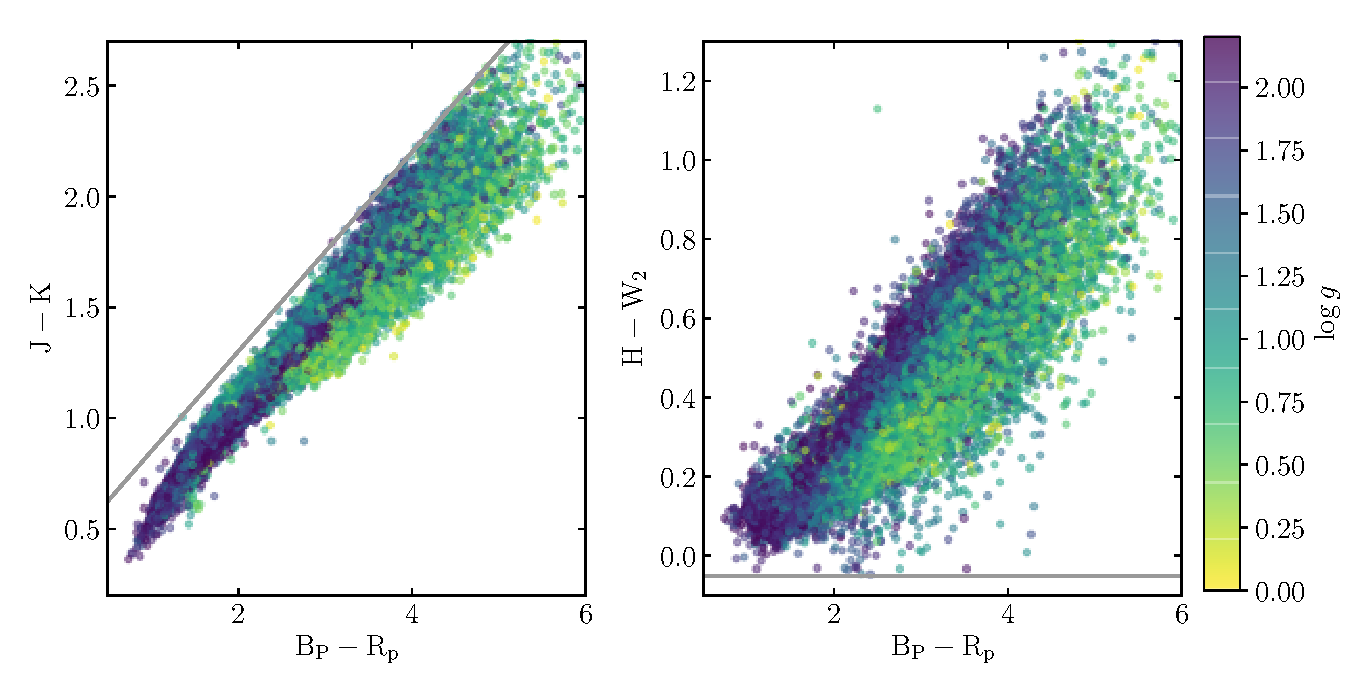
\includegraphics[width=\textwidth]{parent_sample.pdf}
\caption{Color--color diagrams for the Parent Sample stars.
  The points are colored by
  the \apogee\ pipeline estimates of surface gravity.
  The color cuts used to trim outliers are shown as grey lines.\label{fig:parent}}
\end{figure}

Every Parent-Sample star gets, in addition, a randomly assigned binary
label (A or B).
This is used for two-fold validation and jackknife.
In short, we will use the model trained on the A data to assign luminosities
and distances to the B data and \foreign{vice versa}.
The Parent Sample A has HOGG entries and Parent Sample B has HOGG entries.

For training, we need A and B Training Sets.
We define the Training Set stars to be Parent-Sample stars that also
have a measured \gaia\ parallax.
The Training-Set stars, in addition to meeting all Parent-Sample cuts,
also must meet ACE WHAT ADDITIONAL CUTS to ensure that the parallax
measurements are good.
But---as we have emphasized above---we do not cut ever on parallax or
parallax error or their ratio. For this reason, most of the training set
do not have significantly measured parallaxes and HOGG percent even have
negative parallaxes!
But we will perform our training such that it will be unbiased in these
circumstances.
Indeed it would be necessarily biased if ever we did cut on parallax or
parallax signal-to-noise.

In detail,
for each star $n$ in the Training Sets, we take from \gaia\ DR2
the astrometric parallax $\gparallax_n$ and its uncertainty $\sigma_n$.
Importantly, to each \gaia\ parallax measurement we add a positive
offset of $0.029$\,mas to adjust for the under-estimation of
parallaxes reported by the \gaia\ Collaboration (\citealt{lindegren}).
The Training Sets are shown in \figurename~\ref{fig:training}.
\begin{figure}
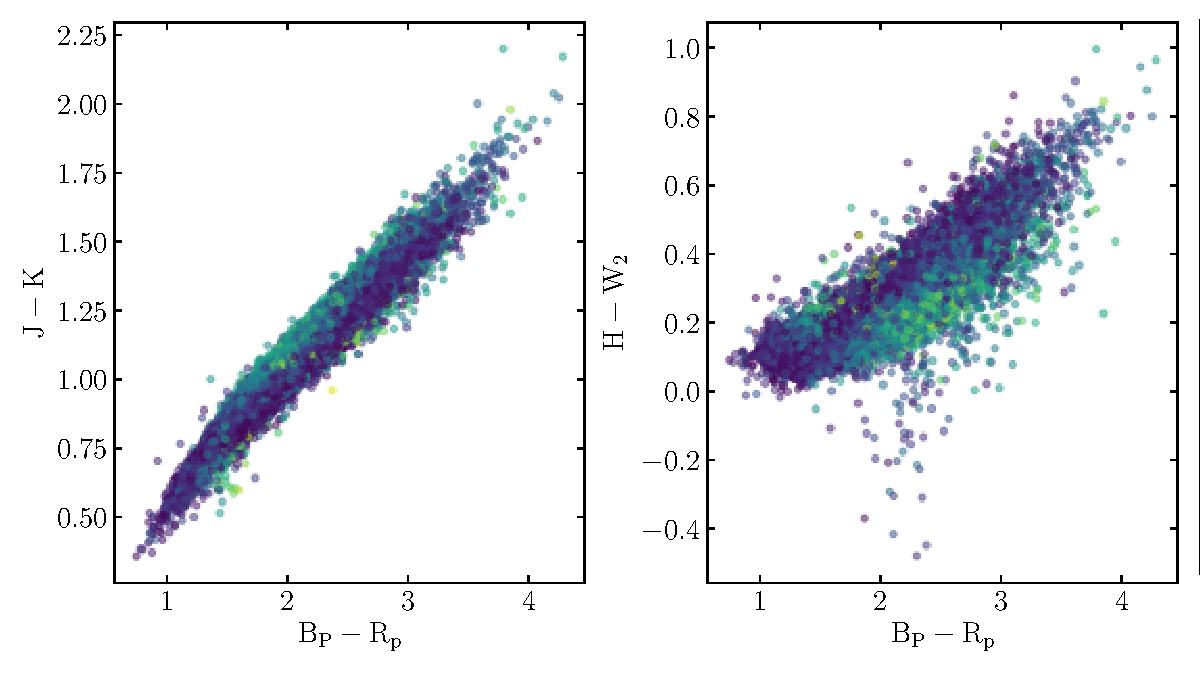
\includegraphics[width=\textwidth]{./training_sample.pdf}
\caption{Color--color diagrams for the Training Set stars.
  Note that there is less color range in the Training Set than in the
  Parent Sample.\label{fig:training}}
\end{figure}

Comparison of {\figurename s}~\ref{fig:parent} and \ref{fig:training} shows
that there is more color range in the Parent Sample than in the Training Set.
This challenges the representativeness assumption in \sectionname~\ref{sec:assumptions}.
The principal reason for the difference is that the \gaia\ quality cuts
exclude stars preferentially from crowded regions, which also tend to be the
most dust-obscured.
The hope of the model assumptions is that the Training Set will contain sufficient
dust variation that the model will naturally learn the dust corrections and extrapolate
acceptably.

For every star $n$ in the full Parent Sample we construct the feature
vector $x_n$ as
\begin{eqnarray}
x_n\T &\equiv& [1, G_n, \BP_n, \RP_n, J_n, H_n, K_n, W_{1n}, W_{2n}, \ln f_{1n}, \ln f_{2n}, \cdots, \ln f_{Ln}]
\quad ,
\end{eqnarray}
where the 1 permits a linear offset,
the photometry is from \gaia, \zmass, and \wise, respectively,
the fluxes in the $L=7405$ \apogee\ spectral pixels (for which there are reliably
and consistently data) for star $n$ are denoted
$f_{1n}$, $f_{2n}$, and so on,
and we have taken logarithms of those fluxes.
These feature vectors live in a $D$-dimensional space where $D=7414$
For every star $n$ in either of the Training Sets we additionally require---in
addition to these feature vectors---a \gaia-measured astrometric parallax $\gparallax_n$
and uncertainty $\sigma_n$.

\section{Results and validation}

We optimize two models, one for Training Set A and one for Training Set B.
The two models are applied to the two splits of the Parent Sample, Parent Sample
A and Parent Sample B, using the A-trained model on Parent Sample B and
\foreign{vice versa}.
For the purposes of assessing the accuracy and precision of the model, this
train-and-test framework constitutes a two-fold cross-validation.
Results of this cross-validation is shown in \figurename~\ref{fig:xval}.
For the stars with highest \gaia-measured parallax signal-to-noise,
the spectrophotometric model is predicting the \gaia\ parallaxes with little bias
and a scatter of better than 9~percent.
\begin{figure}
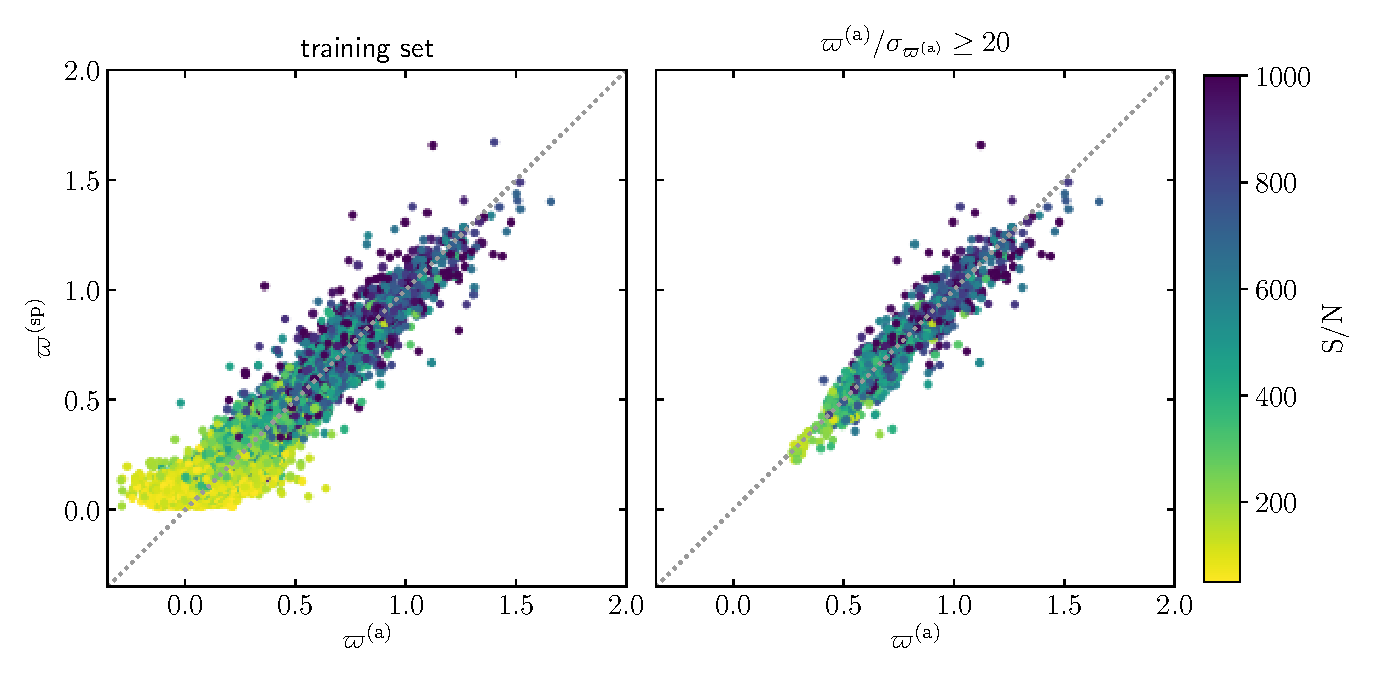
\includegraphics[width=\textwidth]{residuals.pdf}
\caption{The predictive accuracy of the model, in the two-fold cross-validation.
  Each panel shows \gaia\ astrometric parallaxes $\gparallax_n$ on the vertical axis
  and our spectrophotometric parallaxes $\sparallax$ on the horizontal axis.
  The left panel shows the full Parent Sample, the middle panel shows the Training Set
  stars (which pass \gaia\ quality checks; see text), and the right panel shows a
  subset of stars with very high astrometric parallax signal-to-noise. This latter
  set plays no particular role in the method, but it can be used to demonstrate or
  assess the prediction precision. Fractional precision of the prediction
  is XXXX HOGG MEASURED HOW?\label{fig:xval}}
\end{figure}

We used this cross-validation framework to adjust the regularization parameters.
We (arbitrarily) chose zero regularization on the photometric components of the
$x_n$ vectors, and uniform, identical regularization strength for all of the
spectral (\apogee-pixel) components.
We did a coarse grid search in the value for the spectral-component value of the
$\lambda$ vector, using the A/B split as the two-fold cross-validation.
The 9-percent scatter is what we obtain at the optimal setting of the regularization
strength.

We adopt 9~percent as the method's precision.
This estimate is conservative in that the 9-percent scatter includes contributions
from both our spectrophotometric model and from the \gaia\ measurements themselves.
However this estimate is not so conservative in that the test is performed with
\gaia's best stars, which are bright, nearby, in low extinction regions, and
(because of these things) near Solar metallicity.
There could in principle be additional bias or scatter for stars that are in dustier
regions or at lower metallicities.
\figurename~\ref{fig:residuals} shows that
there is no suggestion of any such trends when we color the residuals by metallicity
or $H-W_2$ color (which is a reddening proxy).
\begin{figure}
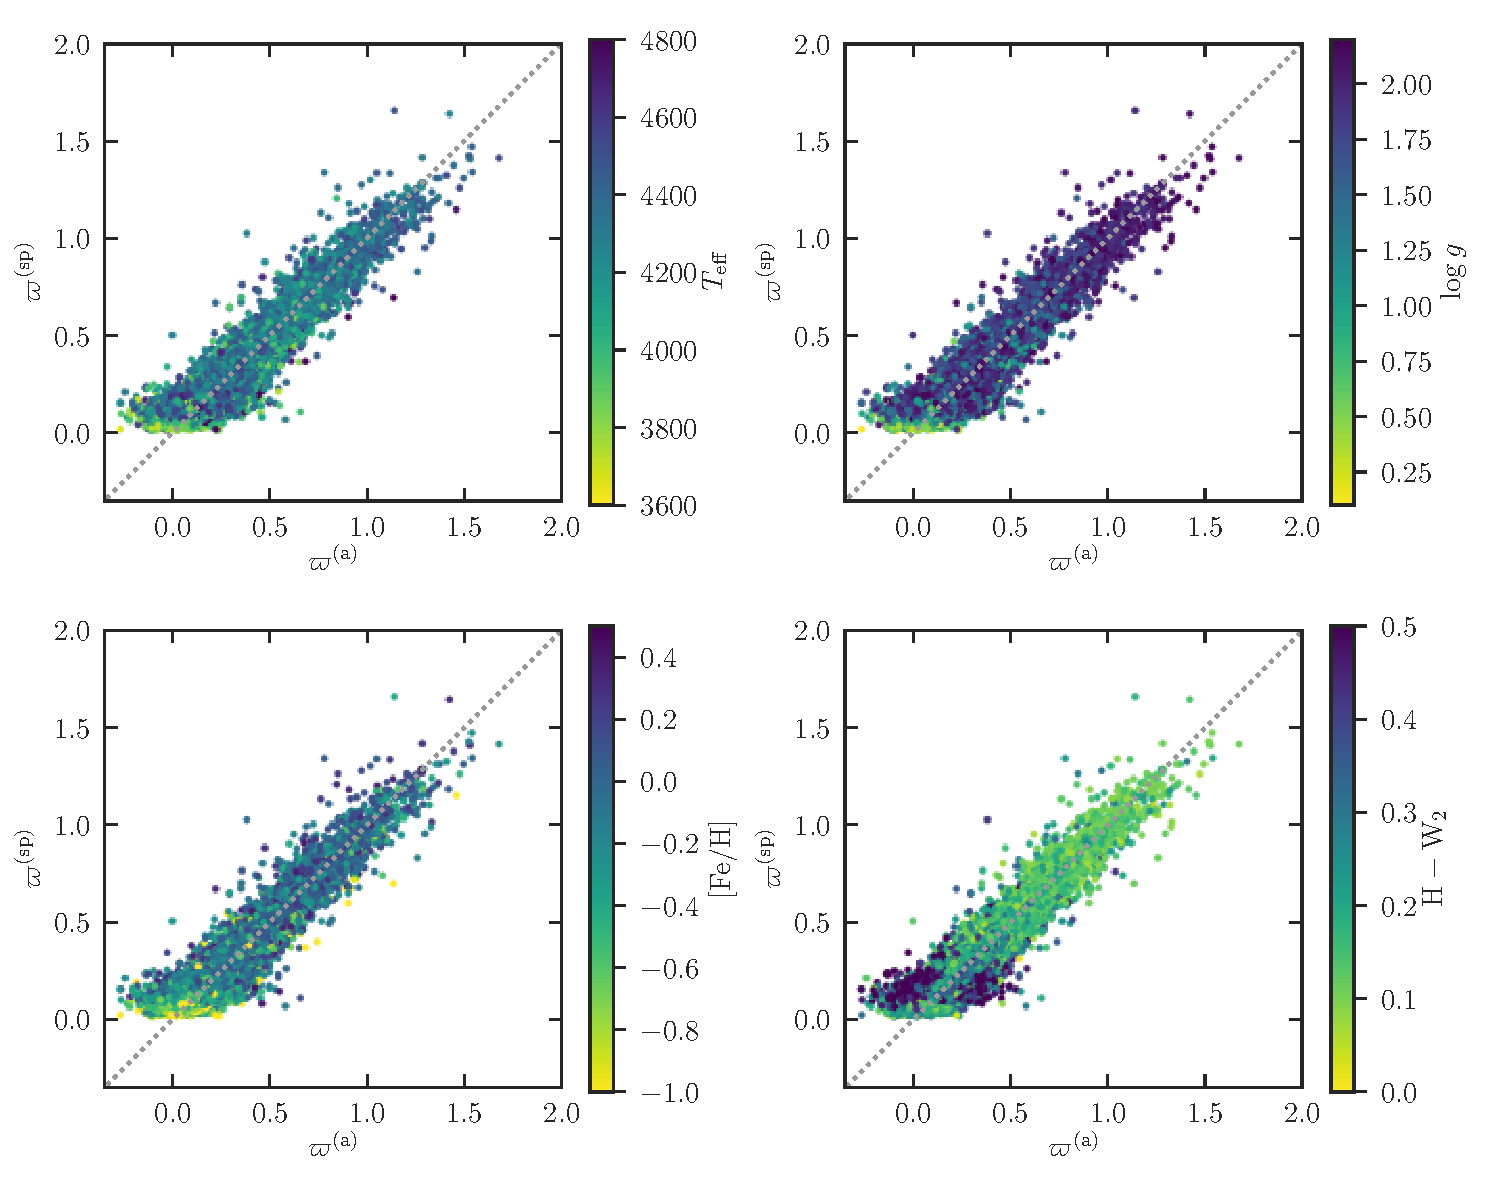
\includegraphics[width=\textwidth]{./residuals_training.pdf}
\caption{Prediction residuals colored by relevant features.
  Each panel shows the prediction residuals (\gaia\ astrometric parallax minus
  spectrophotometric parallax $\gparallax_n-\sparallax_n$) colored by a different
  data feature that might be relevant to the residual.\label{fig:residuals}}
\end{figure}

Another validation of the results can be obtained by looking at known
clusters or spatially compact objects in the data.
In \figurename~\ref{fig:clusters}, we show the parallax distribution from \gaia\ and
the spectrophotometric-parallax distribution from this work for stars in
angular proximity to known stellar clusters and the Sagittarius dwarf
galaxy.
These clusters span some range in metallicity and age, and therefore test
the accuracy of the method for different kinds of populations.
They show that both \gaia\ and the spectrophotometric parallaxes appear to be unbiased
for these clusters and the range in abundances and ages they represent.
HOGG: DO WE NEED TO ADDRESS whether why not these clusters show 9-percent spreads?
\begin{figure}
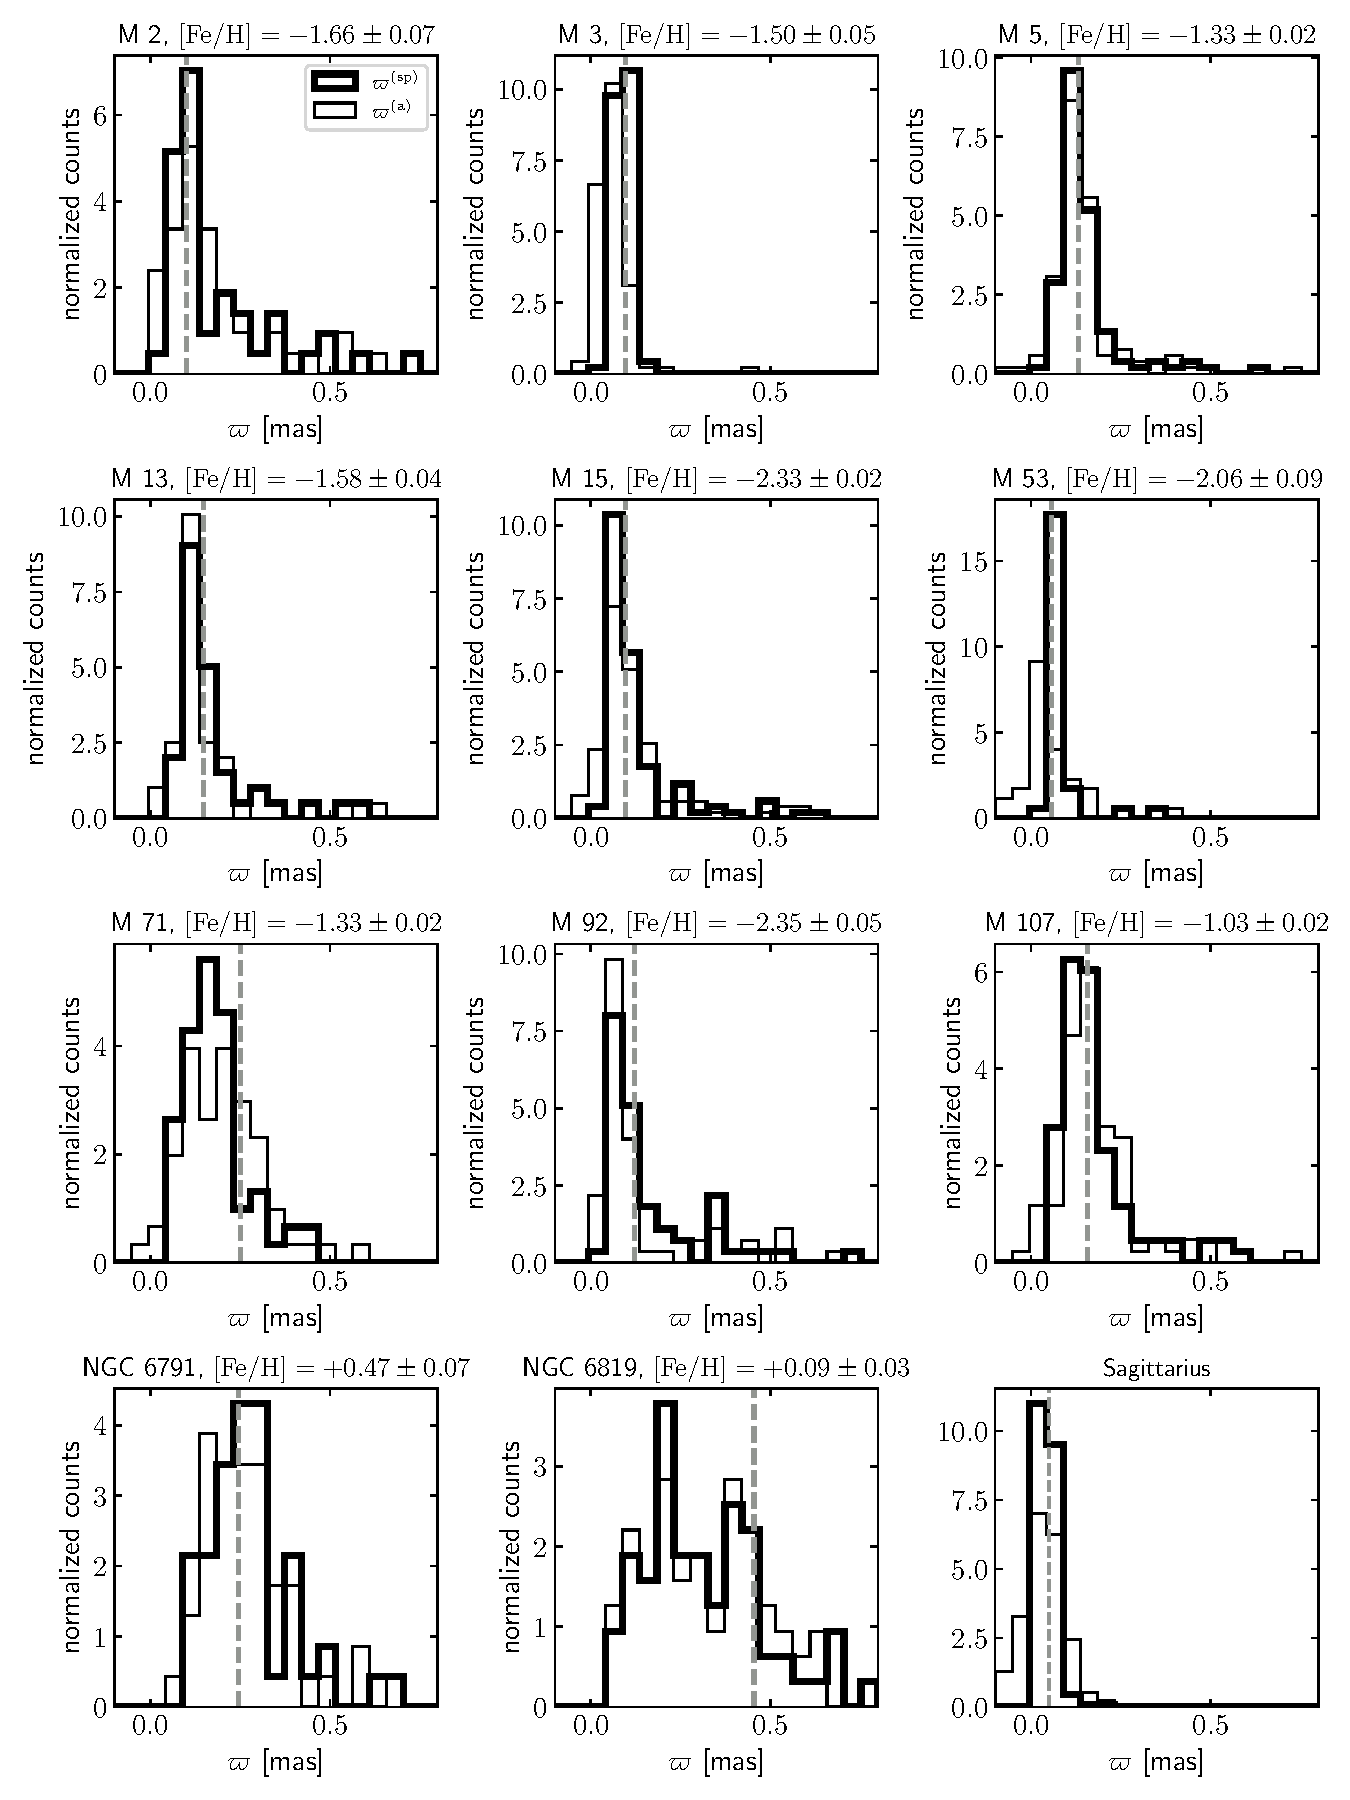
\includegraphics[width=\textwidth]{clusters.pdf}
\caption{The histograms of \gaia\ astrometric parallaxes $\gparallax_n$
  and spectrophotometric parallaxes $\sparallax_n$ for stars in angular proximity
  to various stellar clusters in the \apogee\ observing footprint. In each panel,
  the expected parallax of the cluster is shown as a vertical line.\label{fig:clusters}}
\end{figure}

The linear model we use has a big limitation: Linear models are inflexible.
However, it has a great advantage over more general methods,
which is that it is easy to look inside
the linear model and check whether the dependencies represented there make sense.
The feature vector $x_n$ for star $n$
contains a set of photometry in magnitudes.
Linear combinations of these photometric measurements are like complex synthetic
magnitudes or colors.
Since the model was trained to deliver luminosities of stars given training data
of different metallicities and extinctions, the synthetic photometry developed
by the model should be, in some sense, metallicity- and extinction-independent
photometry for luminous red-giant stars!
In detail this synthetic magnitude is something like HOGG PUT EQUATION HERE AND
SAY SOMETHING ABOUT IT. HOGG: Maybe plot this synthetic photometry against dust
and metallicity.

HOGG: Similarly, the spectral part of the model should also be
interpretable. HOGG DESCRIBE \figurename~\ref{fig:spectral} THAT
DEMONSTRATES THIS, qualitatively.
\begin{figure}
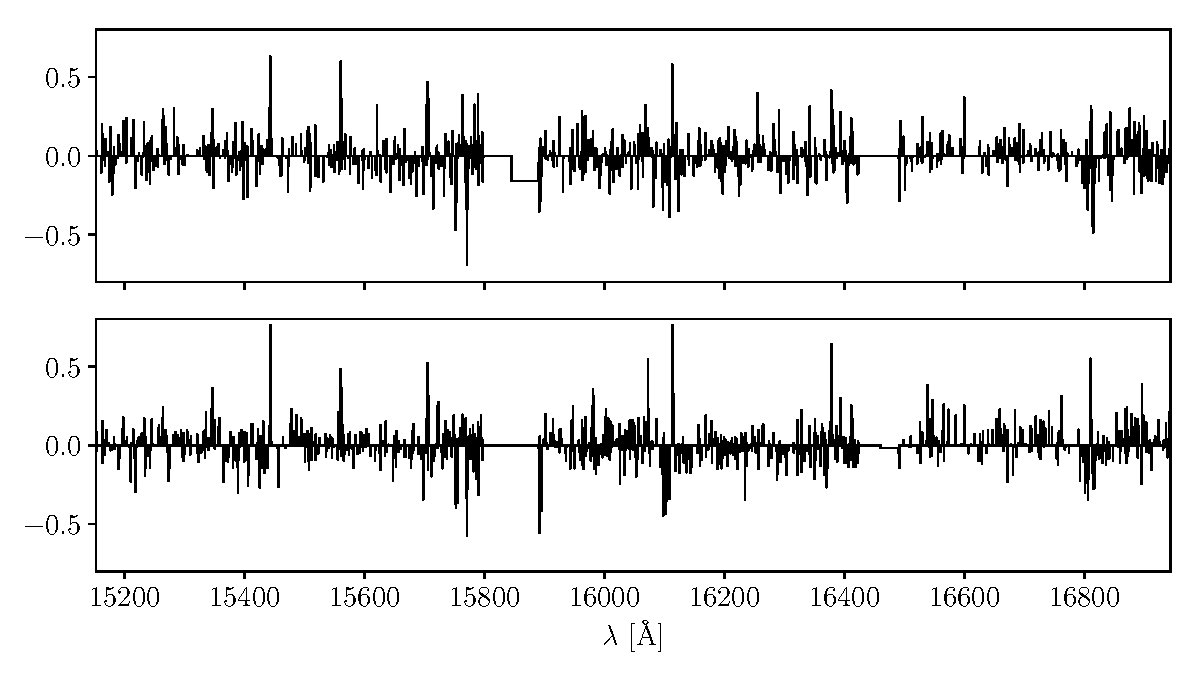
\includegraphics[width=\textwidth]{coefficients.pdf}
\caption{The coefficients of the spectral part of the linear model.
  Also shown are derivatives with respect to labels for a \project{Cannon}-like
  linear regression for the Training Set data.\label{fig:spectral}}
\end{figure}

In the end, this method produces a spectrophotometric parallax estimate $\sparallax_m$ for
every star $m$.
\tablename~\ref{tab:output} shows a snippet of this output, with the full output available
as an electronic data table associated with this \documentname.
In order to use this output with \gaia\ astrometry, we recommend joining the table to the
\gaia\ Catalog on the \zmass\ ID (name), as per the instructions at the \gaia\ Archive (CITE).
In order to use this output with \apogee\ radial velocities and element abundances, we recommend
joining the table to the \sdssiv\ Catalog on the \zmass\ ID (name).
\begin{table}
\caption{The generated spectrophotometric parallaxes.\label{tab:output}}
\end{table}

In order to use these outputs in a probabilistic inference or forward model,
an investigator needs a noise (uncertainty) model.
The linear model permits straightforward propagation of uncertainty from the
feature inputs.
However, these propagated uncertainties clearly under-predict the scatter between
the spectrophotometric parallaxes $\sparallax_m$ and the \gaia\ astrometric
parallaxes $\gparallax_m$.
Our recommendation for an uncertainty model is HOGG WAT?

\section{Discussion}

This project demonstrates that photometry and spectroscopy can be used to predict
or estimate distances to stars.
This isn't new!
However, what's new is that it is possible to do this very well but with a purely
linear model acting on magnitudes and spectral (logarithmic) fluxes, and entirely
data-driven.
That is, a linear model trained on noisy parallax data from \gaia.

The model and method is based on a raft of assumptions, listed above
in \sectionname~\ref{sec:assumptions}.
We make some comments there, but we emphasize some particulars here:

One strong assumption of this work is that our set of features is sufficient to
build a predictive model for distance.
Our arguments for our included features is that they ought to be sufficient to
estimate a dust-independent apparent magnitude and the stellar parameters (especially
age and surface gravity) that are sensitive to luminosity.
In particular, since our model is linear in the logarithm of the parallax, it is
also linear in any kind of apparent magnitude at fixed distance and also linear
in distance modulus at fixed luminosity.
Our feature decisions were highly motivated by these kinds of considerations.
And the derived model parameters shown in \figurename~\ref{fig:spectral} do indicate that
the model is capturing some or all of the expected information in the spectra, at least.

However, our choice of features is very rigid:
In principle the data themselves should tell us what features to include.
In that direction, it would make sense to choose features using a more complex
technique like deep learning or an auto-encoder (CITE).
These methods generate good features automatically.
However, they also involve an enormous set of hyper-parameter-like choices,
and they involve sacrificing certain kinds of interpretability.
However, we expect that a better set of features would do better; in this sense
the project here is just a first step towards precise spectrophotometric distance
estimates.

As we said above, our most restrictive assumption is the linearity assumption.
We required that the parallax prediction be constructed from a linear combination
of the input data or feature vector components.
This is absurd: Stars are not linear objects!
There are two questions to ask about the linearity.
One is: Why did it work? The other is: Could we have done better?
The answer to the first is that we have taken such a small part of stellar parameter
space with our surface gravity cut, that the linearized model of stellar
spectrophotometry is not a bad approximation.
Also, because our linear model included photometry in magnitudes (that is, logarithmic)
and was exponentiated to make the parallax prediction, we knew in advance that much
of the needed flexibility (for dust attenuation, for example) would be close to
linear.
That is, it was a combination of limited model scope and some cleverness in the
feature engineering and model structure.

The answer to the second question is that absolutely we could have done better!
Since models like Gaussian processes and deep networks subsume the linear model
(at least approximately), they could have delivered similar results.
The issues with going to a much more complex model are manifold, however:
We would have had many more decisions to make and many more hyper-parameters
to set.
We would have used some (or maybe much) of the information in the data to learn
the simple fact that the problem is close to linear; that is, if you give a model
a lot of freedom or capacity, it has to use a lot of the data to learn what part
of that capacity it really needs.
A more complex model might have had edge issues: Very flexible models don't extrapolate
outside the convex hull of their training data, and our training data was probably not
balanced in terms of parallax and dust attenuation.
And finally, the complex model would have been harder to visualize and interpret;
the linear model contains essentially only derivatives in the data space, which are
relatively easy to understand.

Although the model, training, and prediction make no use whatsoever about stellar
models, we did use stellar models indirectly to select the Parent Sample of stars:
We used the \apogee\ pipeline (\citealt{aspcap}) surface-gravity $\logg$ measurements.
This tiny use of stellar models could have been obviated by selecting stars not
on the basis of the derived physical parameter, but instead selecting stars to
be similar, observationally, in the spectral space.
That would have lead to a clean sample and made the project independent completely
of stellar models.

One significant limitation of the model is that it does not produce a sensible or
useful noise estimate or error bar on each spectrophotometric parallax estimate.
Although the linear model does permit simple noise propagation, that noise propagation
seriously under-estimates the scatter between the spectrophotometric parallaxes
and the best of the \gaia\ \acronym{DR2} astrometric parallaxes.
We thus used an empirical noise estimate to get our HOGG DETAIL HERE.
In principle it might have been better to build a noise model for our outputs,
and learned that noise model along with the coefficients.

Because of our train-and-test framework, each star is given a spectrophotometric
parallax based on coefficients derived from training on a complementary Training Set sample, of
which that star is not a member.
This framework ensures that the \gaia\ parallax $\gparallax_m$ of star $m$ is never used,
even indirectly, in generating the spectrophotometric parallax $\sparallax_m$ of star $m$.
That means that the parallax estimates generated here and given in \tablename~\ref{tab:output}
is statistically independent of the \gaia\ parallaxes and can be combined with them in
na\"ive ways, for example in inverse-variance-weighted averages.

What is this useful for and how do you use them safely?
HOGG: Show a map of the kinematic rotation of the Galaxy as a function of
x and y, colored by metallicity in \figurename~\ref{fig:disk}.
We see the kinematic center of the Galaxy! We see the rotation curve.
We see the chemical gradients. HOGG WHY CAN YOU NOT JUST READ OFF THINGS FROM THIS PLOT?
\begin{figure}
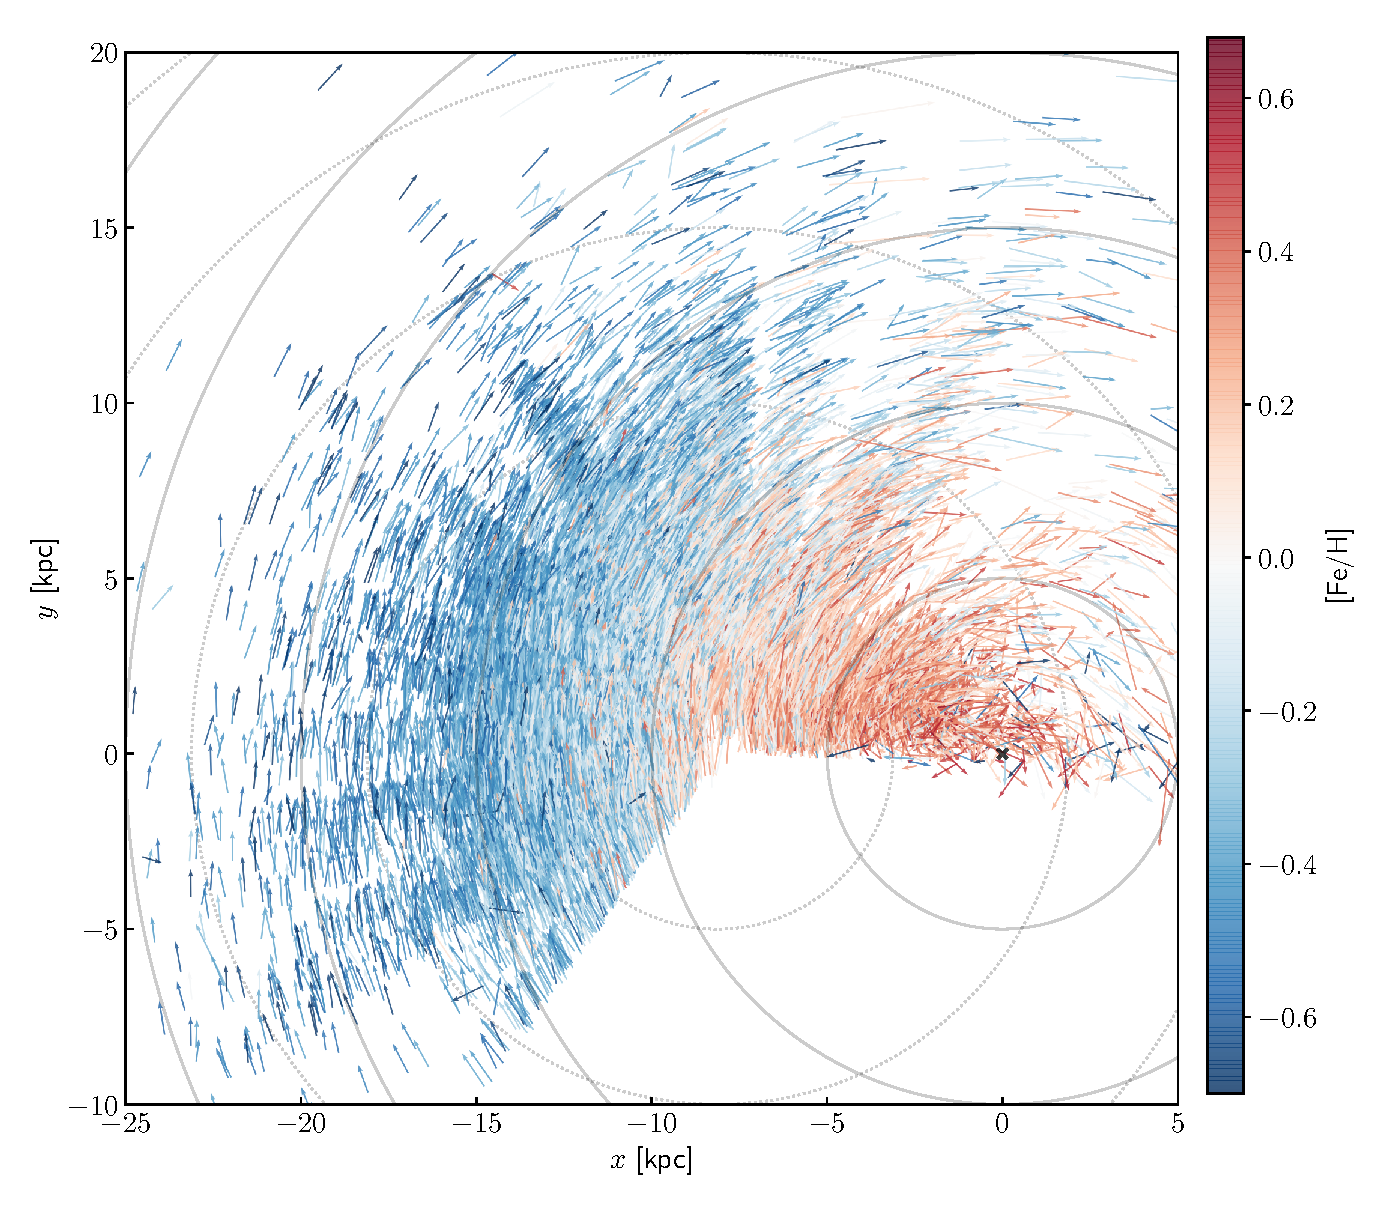
\includegraphics[width=\textwidth]{map.pdf}
\caption{A map of the kinematics and element abundances in the Milky Way disk.
  This map shows the rotation of the Galaxy out to large radius, and also
  indicates the kinematic center of the disk rotation. Interpretation of
  the quantitative information in this plot requires care (see text).\label{fig:disk}}
\end{figure}

\figurename~\ref{fig:disk} shows that this sample of spectrophotometric parallaxes is useful for
mapping the Milky Way.
How does an investigator use these spectrophotometric parallaxes wisely?
How do you build a proper probabilistic model using these?
The answer is similar to the answer to the same question for the \gaia\ \acronym{DR2} data
themselves (\citealt{gaialf}): A likelihood function must be constructed for each of the
spectroscopic parallaxes, given assumptions about the noise in those values.
The sensible likelihood function for star $m$ would be HOGG PUT HERE.
Model fitting can then be built on those likelihood functions.

\acknowledgements
It is a pleasure to thank
  Coryn Bailer-Jones (\acronym{MPIA}),
  Sven Buder (\acronym{MPIA}),
  Andy L. Jones,
  Daniel Michalik (\acronym{ESTEC}),
  Melissa Ness (Columbia),
  and the participants in the \acronym{MPIA} Milky Way Group Meeting
for help with this project.
This project was developed in part at the
2018 \acronym{NYC} Gaia Sprint, hosted by the Center for Computational Astrophysics of
the Flatiron Institute in New York City in 2018 June.

This work has made use of data from the European Space Agency (\acronym{ESA}) mission
\gaia\ (\url{https://www.cosmos.esa.int/gaia}), processed by the \gaia\ Data
Processing and Analysis Consortium (\acronym{DPAC},
\url{https://www.cosmos.esa.int/web/gaia/dpac/consortium}). Funding for the
\acronym{DPAC}
has been provided by national institutions, in particular the institutions
participating in the \gaia\ Multilateral Agreement.

This publication makes use of data products from the Two Micron All Sky Survey, which is a joint project of the University of Massachusetts and the Infrared Processing and Analysis Center/California Institute of Technology, funded by the National Aeronautics and Space Administration and the National Science Foundation.

This publication makes use of data products from the Wide-field Infrared Survey Explorer, which is a joint project of the University of California, Los Angeles, and the Jet Propulsion Laboratory/California Institute of Technology, funded by the National Aeronautics and Space Administration.

Funding for the \project{Sloan Digital Sky Survey IV} has been provided by the Alfred P. Sloan Foundation, the U.S Department of Energy Office of Science, and the Participating Institutions. \sdssiv\ acknowledges
support and resources from the Center for High-Performance Computing at
the University of Utah. The \project{\acronym{SDSS}} web site is \url{www.sdss.org}.

\sdssiv\ is managed by the Astrophysical Research Consortium for the 
Participating Institutions of the \project{\acronym{SDSS}} Collaboration including the 
Brazilian Participation Group, the Carnegie Institution for Science, 
Carnegie Mellon University, the Chilean Participation Group, the French Participation Group, Harvard-Smithsonian Center for Astrophysics, 
Instituto de Astrof\'isica de Canarias, The Johns Hopkins University, 
Kavli Institute for the Physics and Mathematics of the Universe / 
University of Tokyo, the Korean Participation Group, Lawrence Berkeley National Laboratory, 
Leibniz Institut f\"ur Astrophysik Potsdam,  
Max-Planck-Institut f\"ur Astronomie (Heidelberg), 
Max-Planck-Institut f\"ur Astrophysik (Garching), 
Max-Planck-Institut f\"ur Extraterrestrische Physik, 
National Astronomical Observatories of China, New Mexico State University, 
New York University, University of Notre Dame, 
Observat\'ario Nacional~/~\acronym{MCTI}, The Ohio State University, 
Pennsylvania State University, Shanghai Astronomical Observatory, 
United Kingdom Participation Group,
Universidad Nacional Aut\'onoma de M\'exico, University of Arizona, 
University of Colorado Boulder, University of Oxford, University of Portsmouth, 
University of Utah, University of Virginia, University of Washington, University of Wisconsin, 
Vanderbilt University, and Yale University.

\facilities{
\sdssiv(\apogee-2),
\gaia,
\zmass,
\wise}

\software{
\code{Astropy} \citep{astropy, astropy2},
\code{IPython} \citep{ipython},
\code{matplotlib} \citep{matplotlib},
\code{numpy} \citep{numpy},
\code{scipy} \citep{scipy}}

\begin{thebibliography}{}
\bibitem[Abolfathi \etal(2018)]{dr14} Abolfathi, B., Aguado, D.~S., Aguilar, G., \etal\ 2018, \apjs, 235, 42 
\bibitem[Allende Prieto \etal(2008)]{aapogee} Allende Prieto, C., Majewski, S.~R., Schiavon, R., \etal\ 2008, Astronomische Nachrichten, 329, 1018 
\bibitem[Astropy Collaboration \etal(2013)]{astropy} Astropy Collaboration, Robitaille, T.~P., Tollerud, E.~J., \etal\ 2013, \aap, 558, A33 
\bibitem[Astropy Collaboration \etal(2018)]{astropy2} The Astropy Collaboration, Price-Whelan, A.~M., Sip{\H o}cz, B.~M., \etal\ 2018, arXiv:1801.02634 
\bibitem[Bailer-Jones \etal(2018)]{calj} Bailer-Jones, C.~A.~L., Rybizki, J., Fouesneau, M., Mantelet, G., \& Andrae, R.\ 2018, \aj, 156, 58 
\bibitem[Blanton \etal(2017)]{sdssiv} Blanton, M.~R., Bershady, M.~A., Abolfathi, B., \etal\ 2017, \aj, 154, 28 
\bibitem[Casey \etal(2016)]{casey} Casey, A.~R., Hogg, D.~W., Ness, M., \etal\ 2016, arXiv:1603.03040 
\bibitem[Garc{\'{\i}}a P{\'e}rez \etal(2016)]{aspcap} Garc{\'{\i}}a P{\'e}rez, A.~E., Allende Prieto, C., Holtzman, J.~A., \etal\ 2016, \aj, 151, 144 
\bibitem[Ho \etal(2017)]{ho} Ho, A.~Y.~Q., Ness, M.~K., Hogg, D.~W., \etal\ 2017, \apj, 836, 5 
\bibitem[Hogg(2018)]{gaialf} Hogg, D.~W.\ 2018, arXiv:1804.07766
\bibitem[Hunter(2007)]{matplotlib} Hunter, J.~D.\ 2007, CISE, 9(3), 90
\bibitem[Jones \etal(2001)]{scipy} Jones, E., Oliphant, E., Peterson, P. \etal\ 2001, \url{http://www.scipy.org/}
\bibitem[Kollmeier \etal(2017)]{sdssv} Kollmeier, J.~A., Zasowski, G., Rix, H.-W., \etal\ 2017, arXiv:1711.03234 
\bibitem[Lindegren \etal(2018)]{lindegren} Lindegren, L., Hernandez, J., Bombrun, A., \etal\ 2018, arXiv:1804.09366 
\bibitem[Lutz \& Kelker(1973)]{lk} Lutz, T.~E., \& Kelker, D.~H.\ 1973, \pasp, 85, 573 
\bibitem[Majewski \etal(2017)]{apogee} Majewski, S.~R., Schiavon, R.~P., Frinchaboy, P.~M., \etal\ 2017, \aj, 154, 94 
\bibitem[Marrese \etal(2018)]{xmatch} Marrase, P.~M. \etal\ 2018, in preparation
\bibitem[Martig \etal(2016)]{martig} Martig, M., Fouesneau, M., Rix, H.-W., \etal\ 2016, \mnras, 456, 3655 
\bibitem[Mora \etal(2018)]{gaiaarchive} Mora, A., Gonz{\'a}lez-N{\'u}{\~n}ez, J., Baines, D., \etal\ 2018, IAU Symposium, 330, 35 
\bibitem[Ness \etal(2015)]{cannon} Ness, M., Hogg, D.~W., Rix, H.-W., Ho, A.~Y.~Q., \& Zasowski, G.\ 2015, \apj, 808, 16 
\bibitem[Ness \etal(2016)]{nessage} Ness, M., Hogg, D.~W., Rix, H.-W., \etal\ 2016, \apj, 823, 114 
\bibitem[Ness \etal(2018)]{nessdopp} Ness, M., Rix, H.-W., Hogg, D.~W., \etal\ 2018, \apj, 853, 198 
\bibitem[Oliphant(2006)]{numpy} Oliphant, T.~E.\ 2006, \emph{A guide to NumPy}, Trelgol Publishing
\bibitem[P\'erez \& Granger(2007)]{ipython} P\'erez, F. \& Granger, B.~E.\ 2007, CISE, 9(3), 29
\bibitem[Skrutskie \etal(2006)]{zmass} Skrutskie, M.~F., Cutri, R.~M., Stiening, R., \etal\ 2006, \aj, 131, 1163 
\bibitem[Wilson \etal(2010)]{wapogee} Wilson, J.~C., Hearty, F., Skrutskie, M.~F., \etal\ 2010, \procspie, 7735, 77351C 
\end{thebibliography}

\end{document}
